\section{Sviluppi futuri}
\label{sec:conclusions_section_2}

I possibili sviluppi e campi di utilizzo del framework implementato possono essere tanti.
Dopo aver utilizzato in scenari reali il framework, si è ritenuto di focalizzare gli sviluppi successivi nei seguenti ambiti:
(a) integrazione con dispositivi IoT, (b) progettazione collaborativa, (c) fotorealismo.

\subsection{IoT}
\label{sec:conclusions_section_2_sub_1}
Nel mondo gli oggetti presenti nella vita di tutti i giorni hanno al proprio interno del hardware che consente di interagire
con essi da remoto. Questi dispositivi sono denominati IoT (Internet of Things) e consentono l'estensione su Internet degli
oggetti e dei luoghi reali. Questo ci consente di pensare all'inserimento di metadati all'interno dei plugin implementati,
consentendo all'utente un interazione realtime delle informazioni intriseche al modello.\\

\begin{figure}[htbp] %  figure placement: here, top, bottom, or page
   \centering
   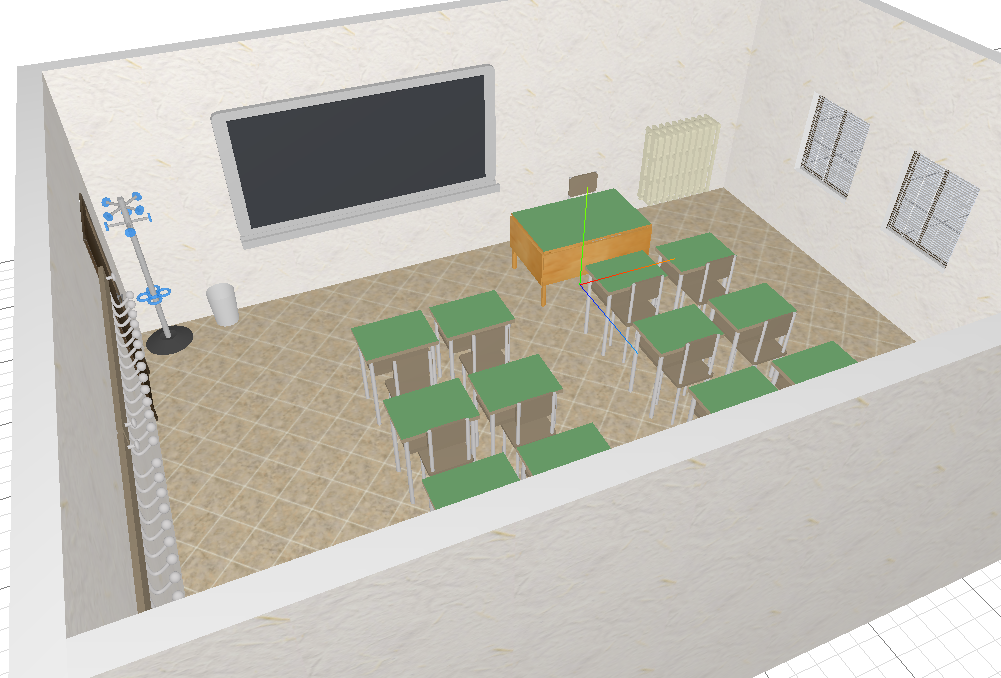
\includegraphics[width=1\linewidth]{images/3d-school-2}
   \caption{PROVVISORIA INSERIRE Immagine Sprite}
   \label{fig:revit}
   \end{figure}
%inserire foto di un plugin con sprite
\newpage

\subsection{Progettazione Collaborativa}
\label{sec:conclusions_section_2_sub_2}
Un altro possibile sviluppo del framework è inserire la modalità di \emph{Progettazione Collaborativa}, consentendo a più utenti
di collaborare contemporaneamente su uno stesso progetto, ottimizando i tempi di lavoro. Si fa riferimento
all'utilizzo all'interno di uno studio di geometri. Lo stack tecnologico scelto per questo sviluppo sono
\emph{Firebase} e \emph{jsondiff}. Il primo è stato scelto(perchè?), per consentire in un possibile sistema di autenticazione degli utenti,
fare un controllo degli accessi e dei permessi al progetto.
Il secondo modulo presente in npm(descrivere npm), consente di confrontare nel contesto collaborativo i file JSON su cui lavorono
gli utenti per trovare le modifiche apportate.\\

% inserire screenshoot
\noindent
\begin{minipage}{.45\textwidth}
\begin{lstlisting}[
                   numbers=left,
                   frame=trBL,
                   basicstyle=\tiny,
                   caption={JSON prima della modifica},
                   label=struttura]
  {
    "id": "HJAe59YF8Ux",
    "x": 201,
    "y": 891,
    "prototype": "vertices",
    "selected": false,
    "lines": ["Hype99FK88x", "S1w-hqKKL8e"],
    "areas": ["Byg1oFKUIe"]
  }
\end{lstlisting}
\end{minipage}\hfill
\begin{minipage}{.45\textwidth}
\begin{lstlisting}[
                   numbers=left,
                   frame=trBL,
                   basicstyle=\tiny,
                   caption={JSON dopo la modifica},
                   label=struttura]
 {
   "id": "HJAe59YF8Ux",
   "x": 201,
   "y": 891,
   "prototype": "vertices",
   "selected": false,
   "lines": ["Hype99FK88x", "S1w-hqKKL8e"],
   "areas": ["Byg1oFKUIe"]
 }
\end{lstlisting}
\end{minipage}

\newpage

\subsection{Fotorealismo}
\label{sec:conclusions_section_2_sub_3}
Con fotorealismo si intende semplicemente che una scena simulata \`e indistinguibile da una fotografia, o per estensione
dalla vita di tutti i giorni. Questo è possibile attraverso la \emph{rasterizzazione}, che consiste in un algoritmo che
permette di convertire un'immagine a due dimensioni in una formata da pixel per avere fotogrammi proiettabili sugli schermi.

% \subsubsection{Baking Service}
Il servizio \emph{Baking} (citazione) \`e un servizio remoto che prende una rappresentazione della scena in JSON come input,
calcola le texture lightmapped, le Mappe Ambientali per riflessione e rifrazione e memorizza le informazioni grafiche
in un formato che \`e compatibile con quello d'ingresso, in modo da permettere l'anello di retroazione di authoring(che significa?).

% The Baking Service is a remote web service that takes a JSON scene representation as its input,
% computes the lightmapped textures, the envmaps for reflections and refractions and stores the enhanced graphic information
%  in a format that is compliant with the input, so enabling the feedback authoring loop.

Lo scopo principale \`e semplificare il workflow durante la visualizzazione 3D per fornire una \emph{User Experience}
ad alto livello sul browser (desktop, tablet e mobile) o su \emph{wearables} come Google Carboard.
Compattare le strutture dati 3D prodotte dall'editor sul browser, trasmetterle ad un servizio di baking web remoto,
e restituire una piacevole esperienza VR in real-time con alto realismo e frame rate. (specificare cosa fa?)
Si stanno sviluppando nuovi algoritmi che portino all'ottimizzazione,
tra cui una soluzione per far fronte a scene di memoria basata su portali e frammentazione del ambienti caricando
su richiesta solo una parte degli interi dati generati.(??????)

\begin{figure}[htbp] %  figure placement: here, top, bottom, or page
   \centering
   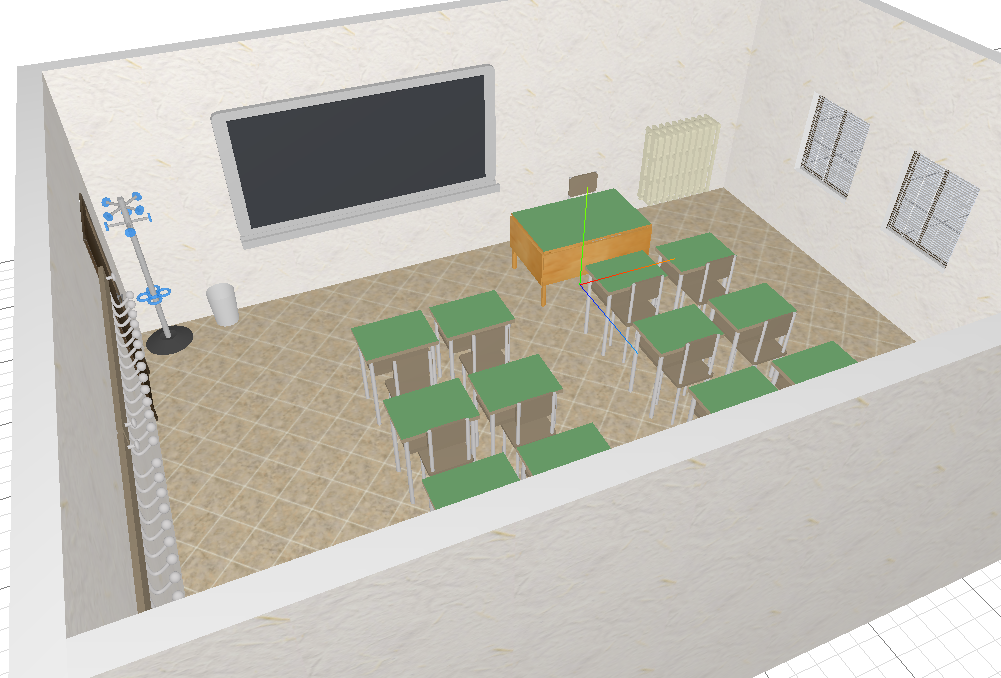
\includegraphics[width=1\linewidth]{images/3d-school-2}
   \caption{PROVVISORIA INSERIRE Immagine Sprite}
   \label{fig:revit}
   \end{figure}
%inserire foto di un plugin con sprite
\newpage

Il fotorealismo può essere esteso in un contesto che fornisce Indoor mapping e indoor/outdoor 3D di modelli realistici
partendo da (a) documenti catastali e/o disegni di costruzione, e (b) scansioni outdoor/indoor realizzate tramite droni
che restituiscono un set di fotografie e di nuvole di punti.
Il possibile range di applicazioni in cui utilizzare il framework spazia dalla sicurezza all'interno di piccole aree o edifici pubblici, a e-commerce,
accesso virtuale al patrimonio culturale, ai videogames, e molto altro ancora.

% In this paper we have discussed a simplified visual 3D workflow to provide a high-level user-experience
%  on web clients (desktop, tablet and mobile, reaching wearables like Google Cardboard).
%  Compact 3D data structures are produced by the editor on the browser, transmitted to a remote web baking service,
%   and given back as a real-time enjoyable VR experience with high realism and frame rate. We are currently providing
%   several optimizations including a solution to cope with out of memory scenes based on portals and fragmentation of
%   the environments, thus loading on demand only a portion of the whole generated data.

 % We are also working to automatize the generation of built environments using the novel LAR (Linear Algebraic Representation)
 %   data structure~\cite{Dicarlo:2014:TNL:2543138.2543294}.

% The project discussed here is actually a component of a much larger programme to provide indoor mapping and indoor/outdoor 3D
%  realistic models starting from (a) cadaster documents and/or building drawings, and (b)  outdoor/indoor drone flights and their
%   returned set of photographs and generated point clouds.
% The possible applications range from security enforcing inside small areas and public buildings, to e-commerce, to virtual access
%  to cultural heritage, to serious games, and much more.

\newpage
